
\documentclass{beamer}

\useoutertheme[height=0.1\paperheight,width=0.1\paperwidth,hideothersubsections]{sidebar}
\usecolortheme{whale}
\usecolortheme{orchid}

\useinnertheme[shadow]{rounded}
\setbeamercolor{title page}{fg=blue!70,bg=blue}
\setbeamercolor{logo}{bg=blue!60}
\setbeamercolor{frametitle}{fg=black,bg=blue!60}
%\setbeamercolor{section in sidebar}{fg=red}
\setbeamercolor{block title}{bg=blue!28!white,fg=blue}
\setbeamercolor{block body}{bg=red!15!white}
\setbeamercolor{sidebar}{bg=blue!70}

\setbeamertemplate{background canvas}[vertical shading][bottom=white,top=blue!25]
\usefonttheme{serif}
\setbeamertemplate{navigation symbols}{}
\usepackage{CJKutf8}
%\usepackage{subfigure}
\usepackage{xmpmulti}
\usepackage{colortbl,dcolumn}
\graphicspath{{November/}}
\DeclareGraphicsRule{*}{mps}{*}{}

\logo{\includegraphics[width=0.1\paperwidth]{huoqiang.jpg}}
\renewcommand{\raggedright}{\leftskip=0pt \rightskip=0pt plus 0cm}
\raggedright
\def\hilite<#1>{\temporal<#1>{\color{blue!35}}{\color{magenta}}{\color{blue!75}}}

\newcolumntype{H}{>{\columncolor{blue!20}}c!{\vrule}}
\newcolumntype{H}{>{\columncolor{blue!20}}c}
\newcommand{\upcite}[1]{\textsuperscript{\cite{#1}}}
\bibliographystyle{plain}
\newcommand{\yihao}{\fontsize{30pt}{\baselineskip}\selectfont}
\newcommand{\sihao}{\fontsize{14pt}{\baselineskip}\selectfont}
\newcommand{\xiaosihao}{\fontsize{12pt}{\baselineskip}\selectfont}
\newcommand{\wuhao}{\fontsize{10.5pt}{\baselineskip}\selectfont}  
\newcommand{\xiaowuhao}{\fontsize{9pt}{\baselineskip}\selectfont} 
\newcommand{\liuhao}{\fontsize{7.875pt}{\baselineskip}\selectfont}
\newcommand{\qihao}{\fontsize{5.25pt}{\baselineskip}\selectfont}
\newcommand{\ThankYouPage}{
  \begin{frame}
    \yihao \centering \textcolor{blue}
    {Thank You!}
  \end{frame}
}

\begin{document}
\begin{CJK*}{UTF8}{gkai}
%  \title{十一月}
%  \author[\textcolor{black}{作者 朱海文}]{作者~~\textcolor{olive}{朱海文}}
%  \institute{\textcolor{violet}{摩科特医疗器械有限公司}}
%  \date{\today}
%  \frame{\titlepage}
%  %======================================================
%  \section*{目录}
%  \frame{\frametitle{目录}\tableofcontents}
%  %========================================
  \begin{frame}\frametitle{统计每一块晶体上泄漏的能量}
    \begin{minipage}[t]{0.2\textwidth}
      \qihao
      右图是每一块晶体上泄漏的能量与击中晶体的能量的比值,一个光子击中探测器多行的事例没有考虑,
      第1行与第24行泄漏的能量没有明显的高于其他行,可能是数据量不够,但如果将每一行泄漏的能量求
      平均值,就可以看到这两行泄漏的能量偏高,见下页。
    \end{minipage}
    \begin{minipage}[t]{0.8\textwidth}
      \begin{figure}[ht]
        \includegraphics[width=\textwidth]{EscapeCrystalRatio.eps}
	\caption{\qihao 每一块晶体上泄漏的能量}
      \end{figure}
    \end{minipage}
  \end{frame}
  %============
  \begin{frame}\frametitle{}
    \begin{figure}[ht]
      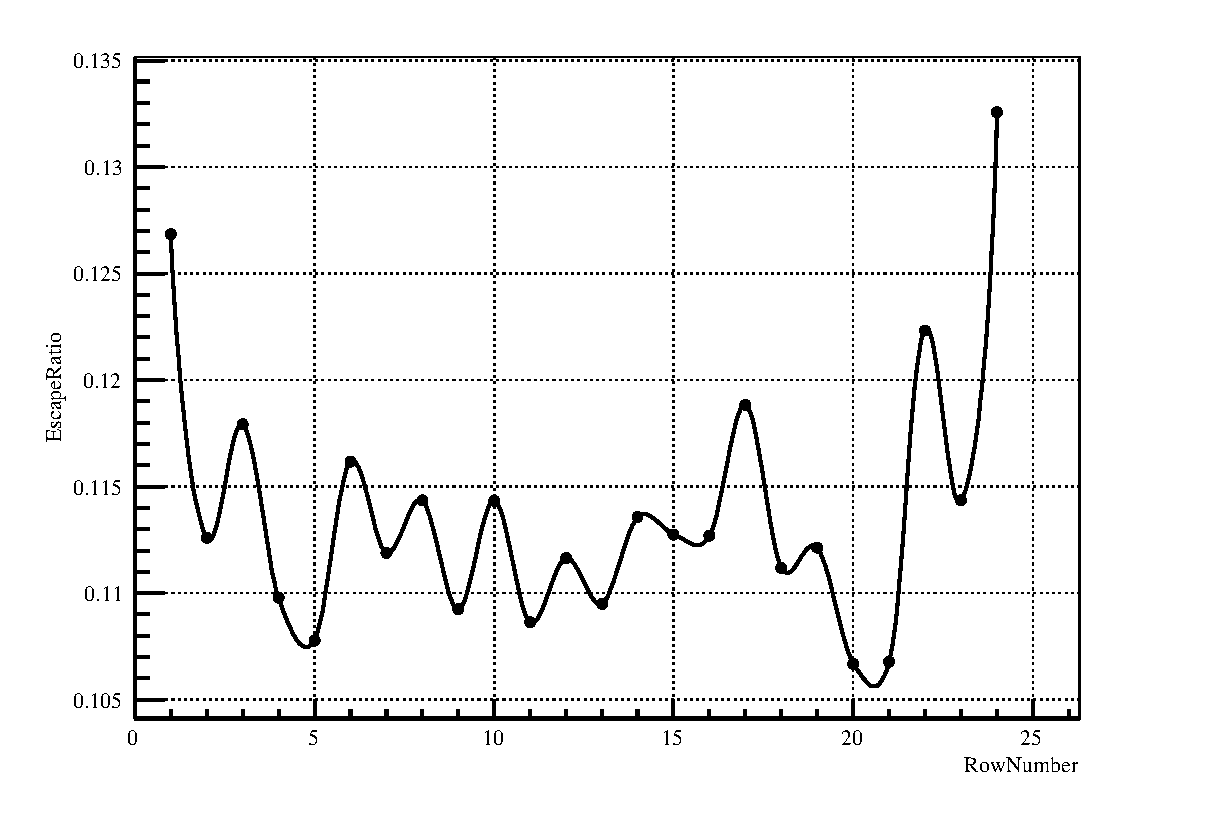
\includegraphics[width=\textwidth]{EscapeRatioNhits1.eps}
      \caption{\qihao 每一行泄漏的能量}
    \end{figure}
  \end{frame}
%=========================================
%  \ThankYouPage
\end{CJK*}
\end{document}
